\begin{figure}
\begin{tabular}{@{}c@{}c@{}}
\begin{subfigure}[b]{0.5\textwidth}
\begin{center}
{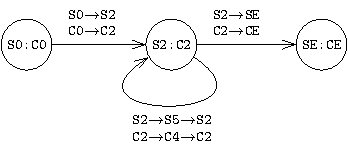
\includegraphics[scale=1.25]{chapters/figures/figSumListProductCfg.pdf}}
\end{center}
\caption{\label{fig:llTraverseProduct}Product-CFG between \cref{fig:llTraverseSpecCFG,fig:llTraverseCCFG}}
\end{subfigure}%
&
\begin{subfigure}[b]{0.5\textwidth}
\begin{center}
\begin{footnotesize}
\begin{tabular}{cl}
\toprule
{\bf PC-Pair} & \multicolumn{1}{c} {\bf Invariants} \\
\toprule
(\scpc{0}{0}) & $\circled{P}\  \sv{l} \indEq{} \lifted{list}{\mem{}}{lnode}{\cv{l}}$ \\
\midrule
\multirow{2}{*}{(\scpc{2}{2})} & $\circled{\scriptsize I1}\  \sv{l} \indEq{} \lifted{list}{\mem{}}{lnode}{\cv{l}}$ \\ &
$\circled{\scriptsize I2}\  \sv{sum} = \cv{sum}$ \\
\midrule
(\scpc{E}{E}) & $\circled{\scriptsize E}\  \sv{ret} = \cv{ret}$ \\
\bottomrule
\end{tabular}
\end{footnotesize}
\end{center}
\caption{\label{fig:llTraverseProductInv}Node invariants for product-CFG in \cref{fig:llTraverseProduct}}
\end{subfigure}%
\\
\end{tabular}
\caption{\label{fig:llTraverseProductCFGInvs}Product-CFG between the CFGs in \cref{fig:llTraverseSpecCFG,fig:llTraverseCCFG}.
\Cref{fig:llTraverseProductInv} contains the corresponding node invariants for the product-CFG.}
\end{figure}
